\documentclass[conference]{IEEEtran}

\usepackage{amsmath}
\usepackage{graphics}
\usepackage{graphicx}

\bibliographystyle{/home/rsheissa/papers/icccas/ieeebib}

\begin{document}

% paper title
\title{A CAD Tool for Automated Design of Low-noise Nullor Based Amplifiers}

% author names and affiliations
\author{Arturo Sarmiento-Reyes, Roberto Casta\~neda-Sheissa, Luis Hern\'andez-Mart\'inez, H\'ector V\'azquez-Leal\\ National Institute for Astrophysics, Optics and Electronics\\
Electronics Department, CAD Group\\ P.O. Box 51, 72000, Puebla, Pue., Mexico}

% make the title area
\maketitle

\begin{abstract}
Low Noise Amplifers (LNA's) have become important for wideband-ultrawideband radio, microwave and cell-phone designers. The nullor represents an ideal active gain, i.e. the plant to be controlled by the feedback network which is usually constituted by passive components.\\
The paper shows that the noise calculation for this passive components and the synthesis of the first stage of the nullor, can be automatically done. This automation is verified by means of a program that designs the feedback network and selects the right device to accomplish noise specs provided by the designer.
\end{abstract}

\section{Introduction}
The design of analogue electronic circuits has often been classified as an art under the assumption that no systematic procedures or methodologies have been developed. Experience has been the major way to produce knowledge regarding analogue design. The traditional way to obtain a new design is by carrying out some modifications on an already existing circuit and made it fulfil some specific features. Nevertheless this way of design results very cryptic and difficult to handle for students.

Structured design has raised as an alternative to accomplish the analog design task. It is based on the concept that the design must start from an ideal solution\--- which obviously fulfils a set of specifications. The structured design is oriented to optimise aspects such as noise, distorion and bandwidth from a block point of view \cite{verhoeven,nordholt}. This approach lets the designer to focus on only one design aspect at a time \cite{stoffels}, such as, noise contributions, distortion aspects or bandwidth.

This work is focused on the first block to be designed which is the noise block. The noise stage will always be the first to be designed because main noise contributions will come from this block. If we consider several blocks like Figure \ref{figure1}; when a resistance is reflected from output to input of the first block, the resistance is diminished by a value equal to the square of the gain. When a resistance is reflected from the output circuit of the second block backwards through two blocks, the resistance is diminished by the product of the squares of the individual gains \cite{vergers}. Therefore, the equivalent noise resistance of the block combination will be given by
\begin{equation}
R_{eq_T}=R_{eq_1}+\frac{R_{eq_2}}{{A_1}^2}+...+\frac{R_{eq_n}}{({A_1}^2)...({A_n}^2)}
\end{equation} 

In fact, this means that main noise contribution will be the first block on the design, so this will be the first stage to synthesize.

\begin{figure}
	\centering
	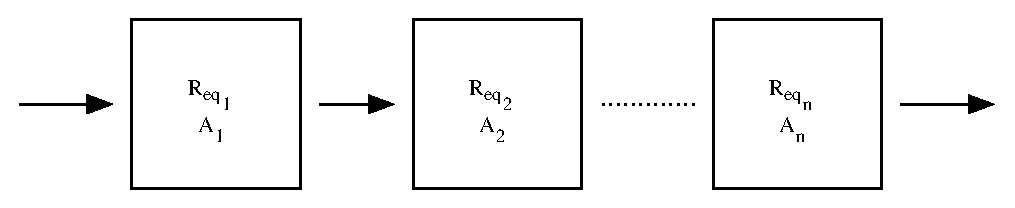
\includegraphics[scale=.55]{figures/amp_blocks.eps}
	\caption{Cascade of multiple stages.}
	\label{figure1}
\end{figure}


\section{Nullor-based amplifiers}
In fact, for the structured design, the nullor constitutes the active (ideal) block of the amplifier. In fact, the nullor is a two-port composed by two elements: {\bfseries \sffamily the nullator} connected at the input port and {\bfseries \sffamily the norator} connected at the output port.

The transmission matrix of the nullor is given as \cite{carlin,moschytz}:
\begin{equation}\label{eq:abcd}
{K}
=
\left [ \begin{array}{cc}
\frac{1}{\mu}& \frac{1}{\gamma} \\\\
\frac{1}{\zeta}& \frac{1}{\beta}
\end{array}
\right ]
=
\left [ \begin{array}{cc}
0 & 0 \\ 0 & 0
\end{array}
\right ]
\end{equation}

It clearly results that the nullor possesses infinite gains for all four transfer relationships, voltage ($\mu$), current ($\alpha$), trans-conductance ($\gamma$) and trans-impedance ($\zeta$).

\begin{figure}
	\centering
	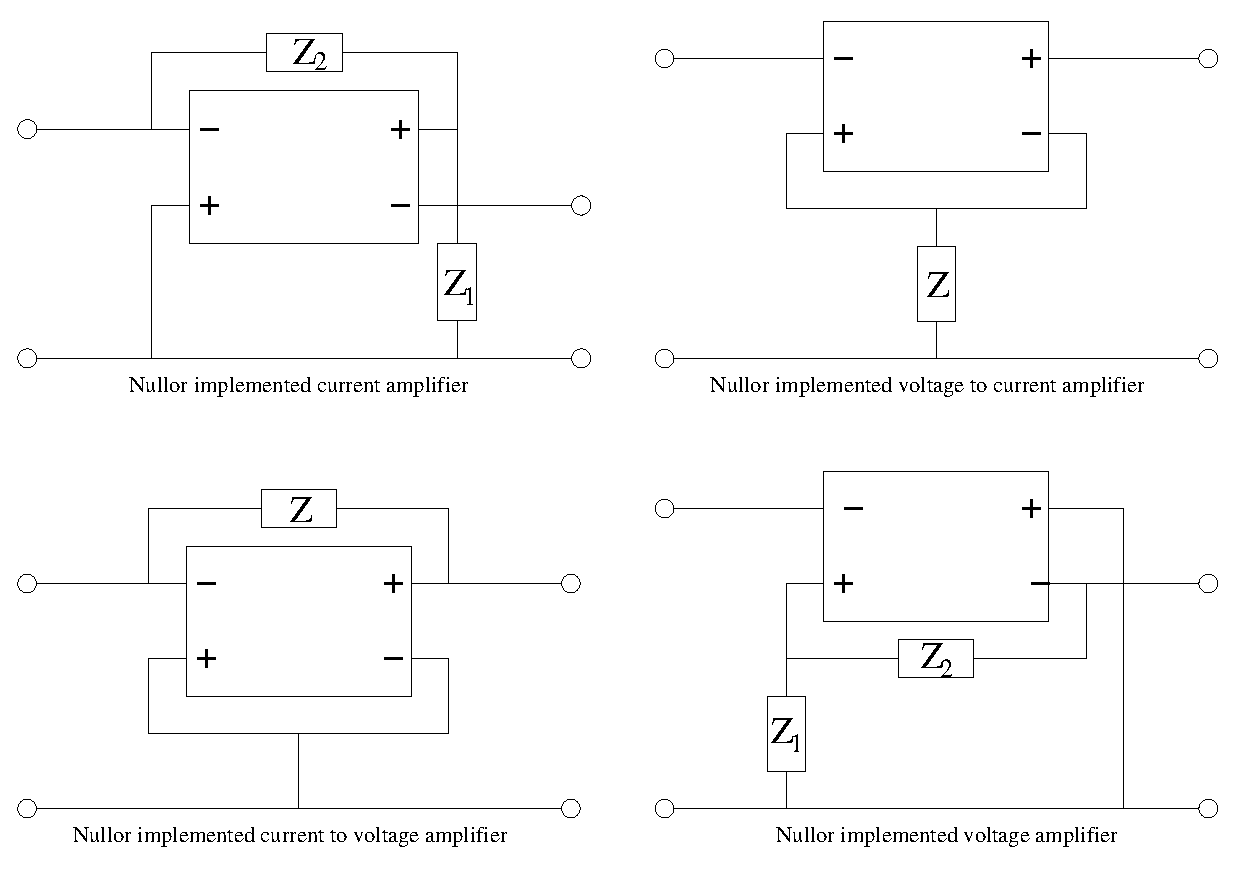
\includegraphics[scale=.4]{figures/nullor_grouped.eps}
	\caption{Negative-feedback Amplifiers.}
	\label{figure2}
\end{figure} 

\begin{figure}
	\centering
	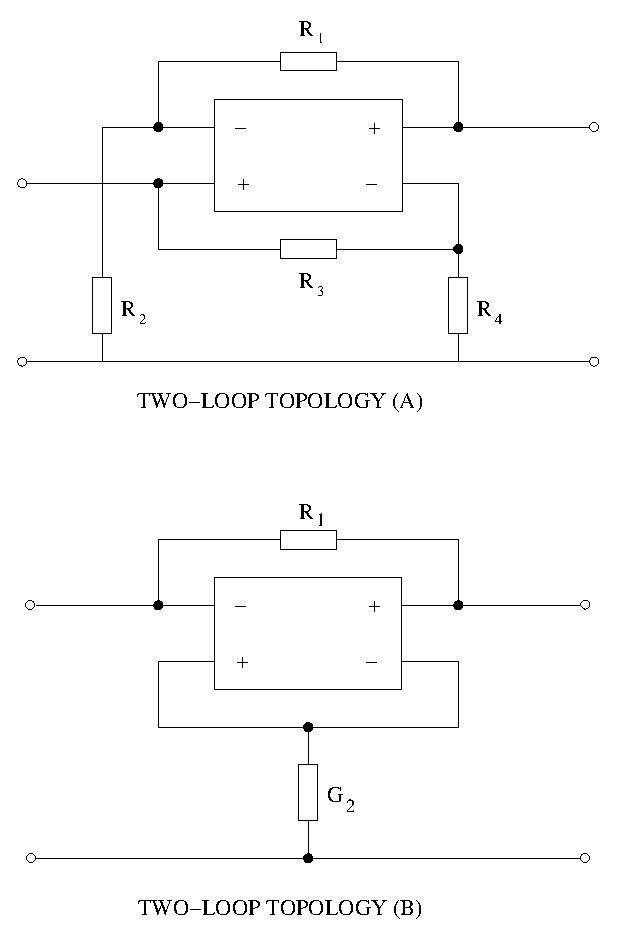
\includegraphics[scale=.55]{figures/basic_two_loops.eps}
	\caption{Two-loop Amplifiers.}
	\label{figure3}
\end{figure}

The basic one-loop amplifiers can be obtained when a passive feedback network is connected with the nullor as shown in Figure \ref{figure2}. If the one-loop amplifiers are combined two new basic two-loop types of amplifiers will be created as shown in Figure \ref{figure3}. The combination of voltage amplifier and current amplifier will be referred as {\bf two-loop topology (A)} and the combination of transconductance and transimpedance amplifiers will be {\bf two-loop topology (B)} \cite{nordholt,stoffels}.

The topology (B) can achieve all four kinds of transfers (voltage, current, transconductance and transimpedance), while topology (A) can achieve all but the transconductance.

\subsection{Noise in the Amplifier}
Noise can be regarded in terms of power spectral densities originated from the passive network and the synthesised nullor. As for the active devices the noise generated is expressed in terms of decibels, this is known as noise figure (NF). Structured design uses power spectral densities for noise calculations then it is necessary to convert the noise figure term for the active devices into a noise voltage and current model, this method is explained in \cite{ott}.

A high-performance feedback amplifier accomplishes a specified transfer of a signal obtained from a signal source with known impedance to a load with known impedance, preserving the quality of the signal as much as possible. The feedback network affects the noise contribution of the noise sources present in the active circuit, usually increasing their contribution. The noise introduced by the transistor stages can be represented by a current and a voltage source placed at the input of the active part. 

Because the structured design constitute in fact the systematic synthesis of the nullor with active devices (BJT of MOS transistors), at the beginning of the design process, a maximum allowable noise values (current and voltage) for the still-to-synthesise nullor must be specified.

The method to obtain the equivalent input noise sources for the single-loop topologies is detailed in \cite{sarmiento}, for the two-loop topologies a similar approach is used although it results rather cumbersome. The overall noise of the amplifier consists of two contributions. A first contribution is originated by the feedback network. A second contribution comes from the active devices. 

In low-noise design JFET's and BJT's are used in the first amplifier stage. MOSFET's are considered less suitable due to their large excess-noise contribution. For each transistor the noise voltage and current are determined by the parameters and the bias current of the transistor \cite{stoffels}. The optimal first stage of the active circuit can be found by determining the optimal bias current. The low noise amplifier is a system where the noise level is carefully handled; it is usually the first block in a radio receiver to amplify the received signal from the antenna with as little distortion and additional noise as possible to be suitable for being processed by the first mixer \cite{svelto}.

Minimisation of noise contribution from active devices is achieved by the calculation of the optimal bias currents. This is done by performing calculations that involve the internal parameters of the device (gm, internal base resistance, collector resistance), the source signal (internal resistance) and the supply source.

\section{Program Development}
The program known as {\bf NOMAD (Noise Optimisation in Modern Amplifier Design)} is a CAD tool aimed to simplify and automate the design process for negative-feedback amplifiers based on nullors. The designer will provide a set of specifications counting of amplifier transfer, configuration, gain, bandwidth and noise level among others.

\begin{figure}
	\centering
	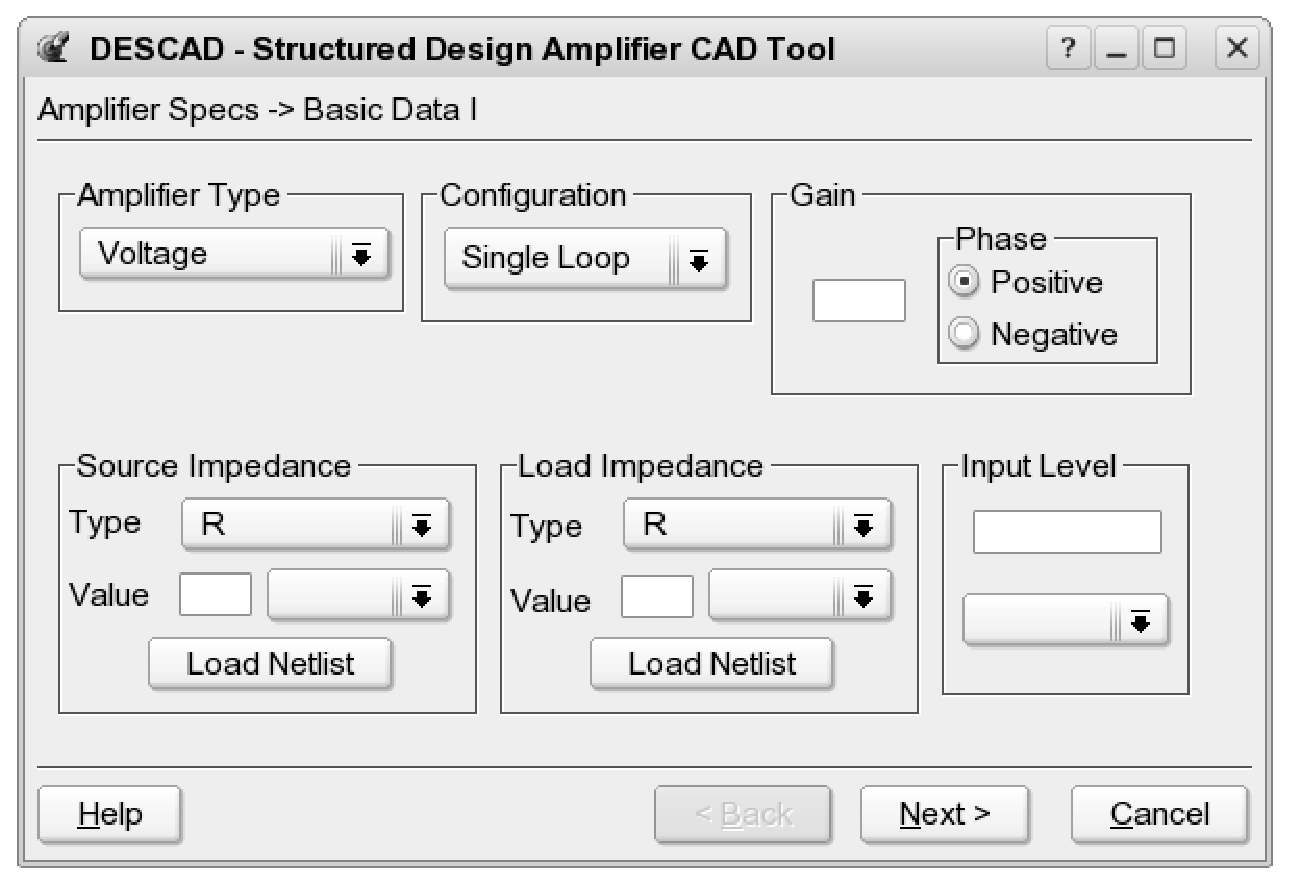
\includegraphics[scale=.4]{figures/descad_1.eps}
	\caption{First screen for NOISECALDC wizard.}
	\label{figure4}
\end{figure}

\begin{figure}
	\centering
	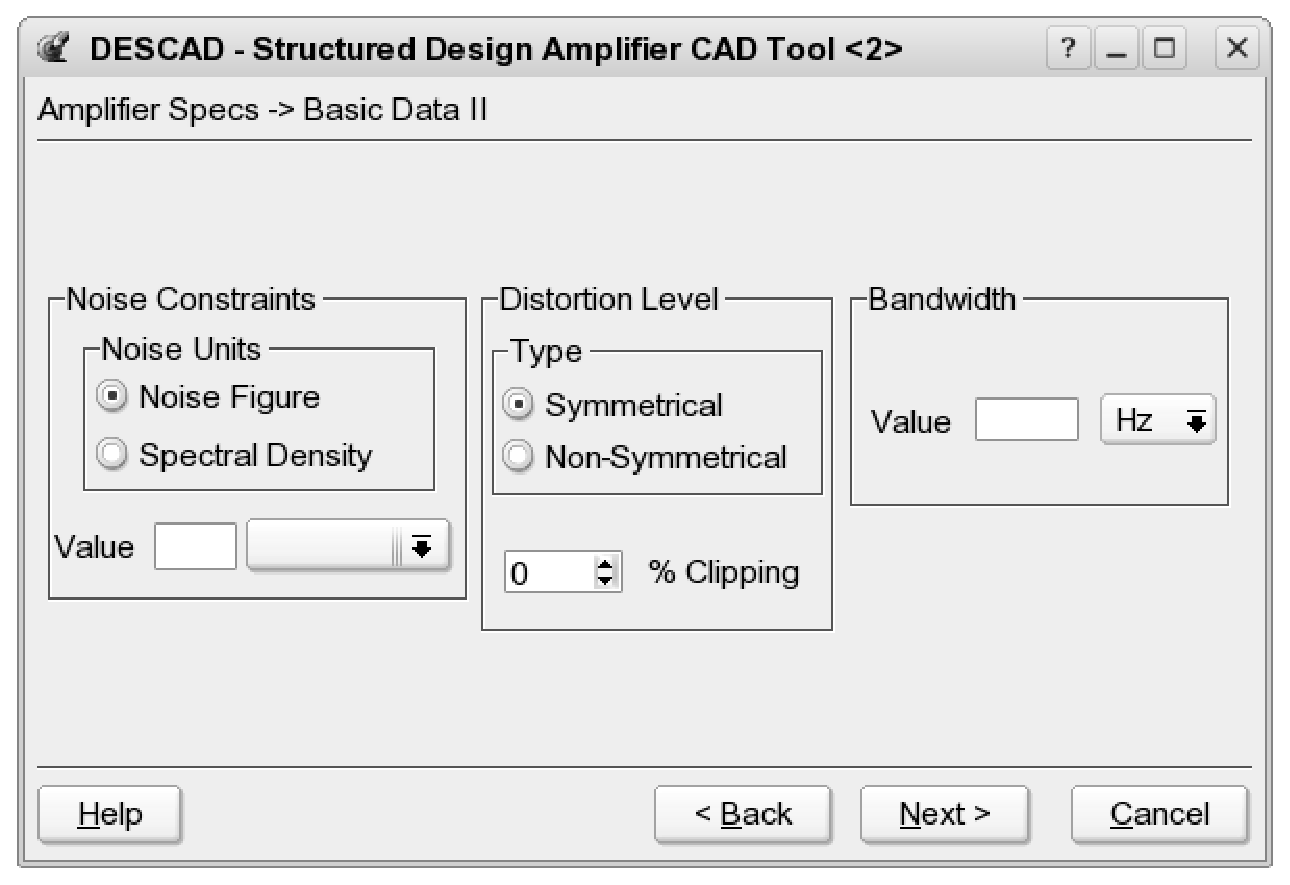
\includegraphics[scale=.4]{figures/descad_2.eps}
	\caption{Second window for NOISECALDC wizard.}
	\label{figure5}
\end{figure}

The tool has been developed in C++ for the backend, while the graphical user interface is programmed in Qt. A primitive version of the tool was developed using Maple \cite{maple1} just for sake of feasibility. The tool is aimed to run under Linux/Solaris without any constraints for special libraries and the Maple package itself, the process has been to port all the equations from Maple to C++.

The main idea about the program is to guide the designer through the design process by means of a wizard approach. This wizard resorts on the use of windows as seen in Figure \ref{figure4}. The first window let the designer select the amplifier type, this is a pulldown menu where a selection could be made between voltage, current, transconductance or transimpedance kind of transfer. Configuration, this is another pulldown menu and choices are single loop, two-loop (A) or two-loop (B). Gain, here the user enter an integer value and selects the output phase (positive or negative). 

Source impedance type, here is a pulldown menu to select a resistive, capacitive, inductive or a circuit type of impedance and its value, the units pulldown menu will have the according units and values, this is, for resistors (ohms, kohms and mohms), capacitors (farad, milifarad, microfarad, nanofarad and picofarad), inductors (henry, milihenry, microhenry, nanohenry). There is another option on the value pulldown menu, {\bf User\_Defined}, this option is when the source impedance will be shaped by more than one element.The last selection is load impedance type, the pulldown menu has the same choices as source impedance (resistive, capacitive, inductive or a circuit) and for the units is the same as load impedance. The empty boxes for source value and load value must be filled in order to continue to the next window, these boxes accept only numbers. 

In case the designer forgets about filling up any box a popup window will warn this situation. Once the program has verified that data has been correctly entered, the designer can press {\bf Next} button and continue to next window.

The Second window \ref{figure5} contains three values to be filled. Distortion will be clipping distortion, this is, the original waveform shape will suffer a cut. The amount of the waveform to be cut is given in percent values. Bandwidth value means the overall bandwidth that amplifier will handle, this is not related to initial and final frequency values. 

Noise value can be given in two different units. Noise figure will be given in decibel units while spectral density is given by $\frac{V}{\sqrt{Hz}}$ or $\frac{A}{\sqrt{Hz}}$, that depends on source units. The bandwidth box must be filled otherwise a warning popup sign will appear. Once all values have been entered and verified, it is possible to continue the process.

Once the basic specs have been provided the program will do the required calculations in order to fulfil them. The first part will be the calculation for the feedback network, this is performed on third window, entitled {\bf Noise, Step 1}. In order to accomplish the overall noise level provided it is necessary to do a tradeoff about the noise from the feedback network and the active device that synthesizes the nullor. 

As seen in Figure \ref{figure6}, the user presses the {\bf Calculate FB Noise} button and the program calculates the required value for the feedback network, this calculation will account for the desired gain value also. The calculated noise values appear under the frame entitled {\bf Noise Values}, here the noise contributions by feedback network and source are shown. 

The box labelled {\bf Required Nullor Synthesized Noise} shows the noise value that the active device must accomplish. In case the resistor(s) noise value(s) produce a large noise value, a warning message will appear. Here the designer must decide to continue or to modify values from previous windows. Once the feedback network noise is acceptable, the next step is to select an active device and its configuration, press the {\bf Next} button. 

\begin{figure}
	\centering
	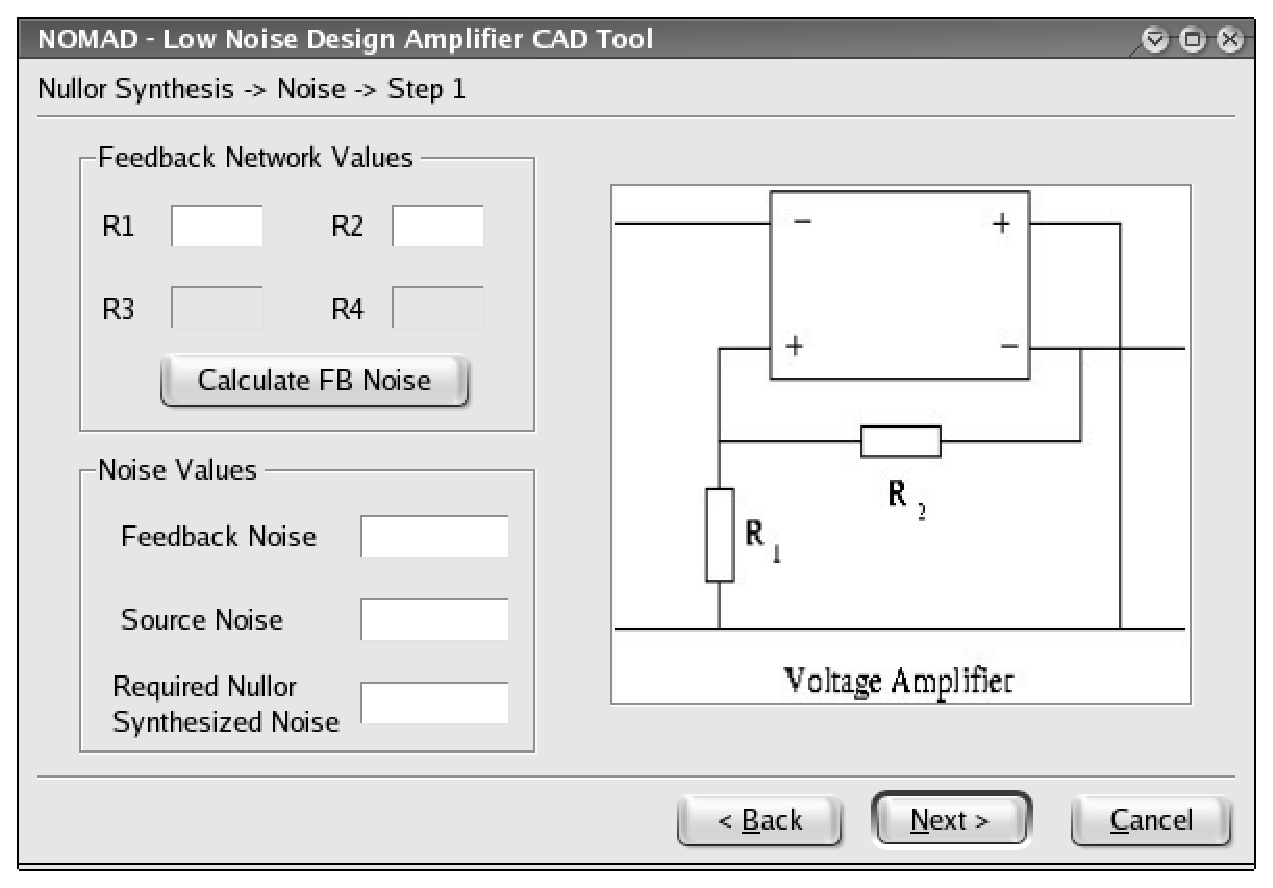
\includegraphics[scale=.4]{figures/descad_3.eps}
	\caption{Feedback noise calculation.}
	\label{figure6}
\end{figure}

\begin{figure}
	\centering
	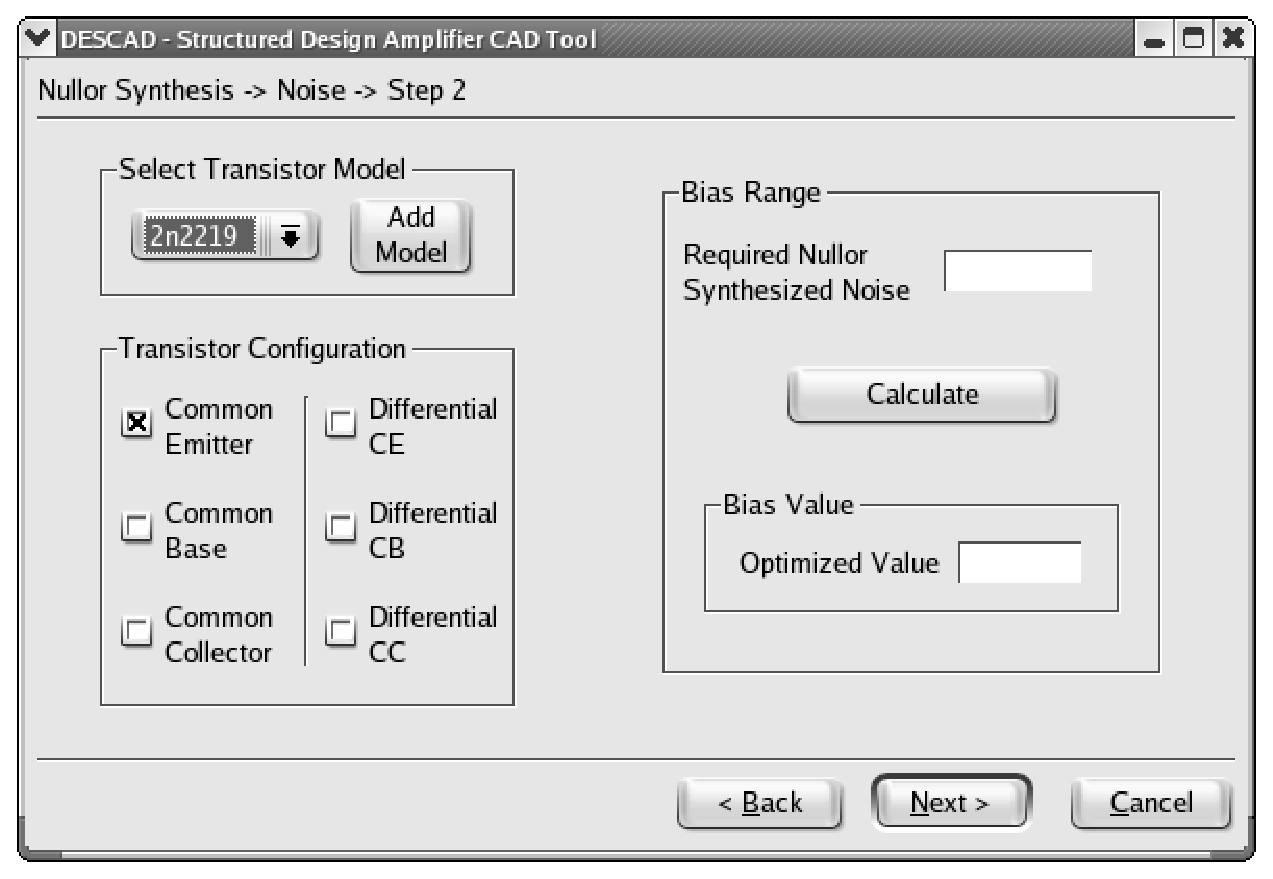
\includegraphics[scale=.4]{figures/descad_4.eps}
	\caption{Active device noise calculation.}
	\label{figure7}
\end{figure}

The Figure \ref{figure7} shows the window entitled {\bf Noise, Step 2}. It has a pulldown menu where designer selects the active device model. Next step is select configuration for this device. These are push buttons with several choices (common emitter, common base, common collector, differential common emitter, differential common base, differential common collector). At this design stage the designer can compare results choosing different combinations. Now it is time to calculate a bias range where the active device can perform within noise limits. This is done pressing the {\bf Calculate} button under {\bf Bias Range}. If everything goes right the minimum and maximum values appear inside boxes labelled {\bf From} and {\bf To} respectively, the designer then must choose a value within these limits to supply the active device. 

In case that not a valid bias range can be calculated,  a warning pop-up window appear indicating that is not possible to calculate a valid bias range. Device selection is made by selecting model numbers, the designer must know if this number belongs to a bipolar or mosfet. If tool fails for second time to accomplish a valid bias range, the design process will begin from the first screen.

For the noise calculations on resistors and active devices SPICE like calculations are performed \cite{spice}. All found equations and the values obtained using them were validated after performing simulations on APLAC \cite{aplac}, this simulation tool includes a model which resembles the nullor behaviour. Once validated these equations, the next task is translate the Maple code to C++ code and perform some tests on the program.

The tool finishes after delivering the final results for the amplifier, i.e. the value of the feedback resistors, the data regarding the active device parameters and the required bias current. This is visualised in a last window of the GUI.

\section{Example}
A design example is provided in order to show the function of the tool. The amplifier to be designed is based on a 1.5 volt 1.5GHz CMOS LNA \cite{lee}. Although this is a CMOS design it will work as a workbench for the tool. The desired gain is 30 and noise figure 6.17dB, the bandwidth to handle will be 10kHz. The basic data for the first screen are entered in Figure \ref{figure4}. Noise, bandwidth and clipping distortion values are entered in Figure \ref{figure5}.

The calculated values for the feedback network are (Figure \ref{figure6}):
\begin{itemize}
\item R1 = 33 $\Omega$
\item R2 = 957 $\Omega$
\end{itemize}

Noise factor is 1.638 or 2.14 dB in noise figure terms, this value represents around the forty percent from the total noise contribution. Next step is to select the active device, configuration and then calculate the adequate bias current.

The selected device is a BJT 2N2222 in common emitter configuration, the selected bias current value is 0.7 mA, recall Figure \ref{figure7}. The noise factor is 2.459 or the noise figure value is 3.907 dB. The total noise figure for the amplifier is 6.047 dB, this means that the tool can compute the adequate values for the resistors and bias value for the active device.

\section{Conclusion}
It has been shown that it is possible to develop a CAD tool capable to automate the design of low noise amplifiers based on a set of specifications provided by the designer. By means of a wizard approach this program makes the designer define step by step his specs. In case that the specs can not be fulfilled, the design process is stopped and taken to a previous step to modify one or more values. When the design process is repeated more than two times because of failure to comply a specification, it will be restarted from the initial step. The development of this program is based entirely on structured design, this shows that this design approach can speed up the design process obtaining accurate results. This tool can be applied not only to low noise amplifiers but to designs that not require so tight requirements by choosing larger values for noise or narrowing bandwidth.

\section*{Acknowledgement}
Roberto Casta\~neda Sheissa is holder of a scholarship from CONACyT M\'exico under contract 118652/120341. This work has been partially supported by a CONACyT M\'exico research project under grant 42588-Y.


\bibliography{bib/icccas}
\end{document}


